\documentclass[10pt,a4paper, margin=1in]{article}
\usepackage{fullpage}
\usepackage{amsfonts, amsmath, pifont}
\usepackage{amsthm}
\usepackage{graphicx}
\usepackage{float}

\usepackage{pdfpages}
\usepackage{minted}

\usepackage{tkz-euclide}
\usepackage{tikz}
\usepackage{pgfplots}
\pgfplotsset{compat=1.13}

\usepackage{geometry}
 \geometry{
 a4paper,
 total={210mm,297mm},
 left=10mm,
 right=10mm,
 top=10mm,
 bottom=10mm,
 }
 % Write both of your names here. Fill exxxxxxx with your ceng mail address.
 \author{
  Çavuşoğlu, Arda\\
  \texttt{e2448249@ceng.metu.edu.tr}
  \and
  Çolak, Eren\\
  \texttt{e2587921@ceng.metu.edu.tr}
}

\title{CENG 384 - Signals and Systems for Computer Engineers \\
Spring 2023 \\
Homework 1}
\begin{document}
\maketitle



\noindent\rule{19cm}{1.2pt}

\begin{enumerate}

\item %write the solution of q1
    \begin{enumerate}
    % Write your solutions in the following items.
    \item %write the solution of q1a
        $z = x + yj \hspace{1cm} 2z+5 = j-\Bar{z} \vspace{0.2cm}\\$
        $2x+2yj+5=j-(x-yj) \vspace{0.2cm}\\$
        $3x+5+yj=j \hspace{1cm} y=1, x=\frac{-5}{3}, z=\frac{-5}{3}+j \vspace{0.2cm}\\$
        $|z|^2 = \frac{34}{9}\\$

        \begin{tikzpicture}
            \begin{axis}[
                title={z},
                axis x line=center,
                axis y line=center,
                xlabel={Real},
                ylabel={Imaginary},
                xmin=-2, xmax=2,
                ymin=-2, ymax=2,
                xtick={-2,-1,0,1,2},
                ytick={-2,-5/3,-1,0,1,2},
                xmajorgrids=true,
                ymajorgrids=true,
                grid style=dashed,
            ]

            \addplot[
                color=blue,
                mark=square,
            ]
            coordinates {
                (0,0)(1,-5/3)
            };
    
            \end{axis}
        \end{tikzpicture}\\
    


        
        
    \item %write the solution of q1b
        $z = r.e^{j\Theta} \hspace{1cm} z^5 = 32j \vspace{0.2cm}\\$
        $j=e^{\frac{\pi}{2}j} \hspace{1cm} r^5e^{5\Theta j}=32e^{\frac{\pi}{2}j} \hspace{1cm} r=2, \Theta = \frac{\pi}{10}, z=2e^{\frac{\pi}{10}j}\\$
    
    \item %write the solution of q1c
        $(1+j) = \sqrt{2}.e^{\frac{\pi}{4}j} \vspace{0.2cm}\\$
        $(\frac{1}{2}+\frac{\sqrt{3}}{2}j) = e^{\frac{\pi}{3}j} \vspace{0.2cm}\\$
        $(-1+j) = \sqrt{2}.e^{\frac{3\pi}{4}j} \vspace{0.2cm}\\$
        $\frac{\sqrt{2}.e^{\frac{\pi}{4}j}e^{\frac{\pi}{3}j}}{\sqrt{2}.e^{\frac{3\pi}{4}}} = e^{\frac{-2\pi}{3}j} \vspace{0.2cm}\\$
        $r = 1, \Theta = \frac{-2\pi}{3}\\$
    
    \item %write the solution of q1d
        $z = j.e^{-j.\frac{\pi}{2}} \hspace{1cm} j = e^{\frac{\pi}{2}.j} \vspace{0.2cm}\\$
        $z  =e^{\frac{\pi}{2.}j}.e^{\frac{-\pi}{2}.j} = 1 = e^{2\pi j}\\$
        
    \end{enumerate}

\vspace{4cm}
\item %write the solution of q2 
    $x(t) \longrightarrow \vspace{-4cm}\\$ 
    \hspace*{2cm} 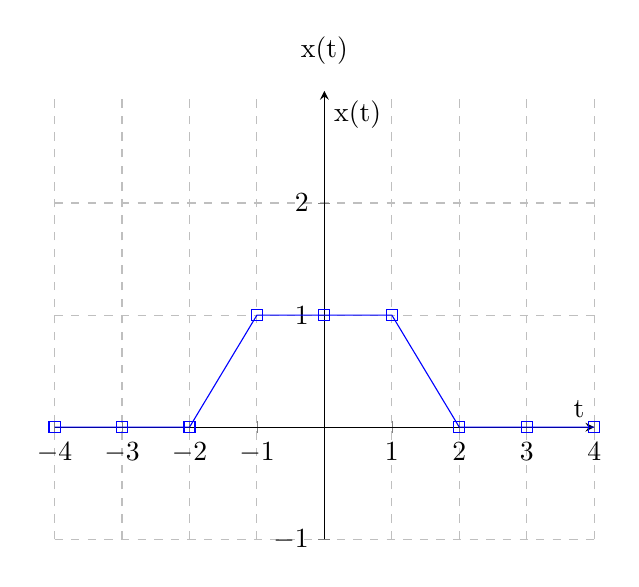
\begin{tikzpicture}
        \begin{axis}[
            title={x(t)},
            axis x line=center,
            axis y line=center,
            xlabel={t},
            ylabel={x(t)},
            xmin=-4, xmax=4,
            ymin=-1, ymax=3,
            xtick={-4,-3,-2,-1,0,1,2,3,4},
            ytick={-2,-1,0,1,2},
            xmajorgrids=true,
            ymajorgrids=true,
            grid style=dashed,
        ]

        \addplot[
            color=blue,
            mark=square,
        ]
        coordinates {
            (-4,0)(-3,0)(-2,0)(-1,1)(0,1)(1,1)(2,0)(3,0)(4,0)
        };
    
        \end{axis}
    \end{tikzpicture}\vspace{3.5cm}\\
    

    $x(t+2) \longrightarrow \vspace{-4cm}\\$ 
    \hspace*{2cm} 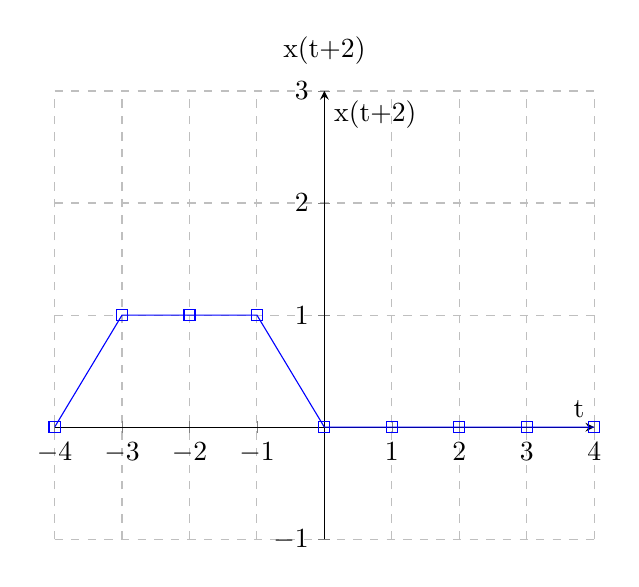
\begin{tikzpicture}
        \begin{axis}[
            title={x(t+2)},
            axis x line=center,
            axis y line=center,
            xlabel={t},
            ylabel={x(t+2)},
            xmin=-4, xmax=4,
            ymin=-1, ymax=3,
            xtick={-4,-3,-2,-1,0,1,2,3,4},
            ytick={-1,0,1,2,3},
            xmajorgrids=true,
            ymajorgrids=true,
            grid style=dashed,
        ]

        \addplot[
            color=blue,
            mark=square,
        ]
        coordinates {
            (-4,0)(-3,1)(-2,1)(-1,1)(0,0)(1,0)(2,0)(3,0)(4,0)
        };
    
        \end{axis}
    \end{tikzpicture}\vspace{4cm}\\



    $x(\frac{t+2}{2}) = x(\frac{t}{2}+1) \longrightarrow \vspace{-4cm}\\$ 
    \hspace*{4cm} 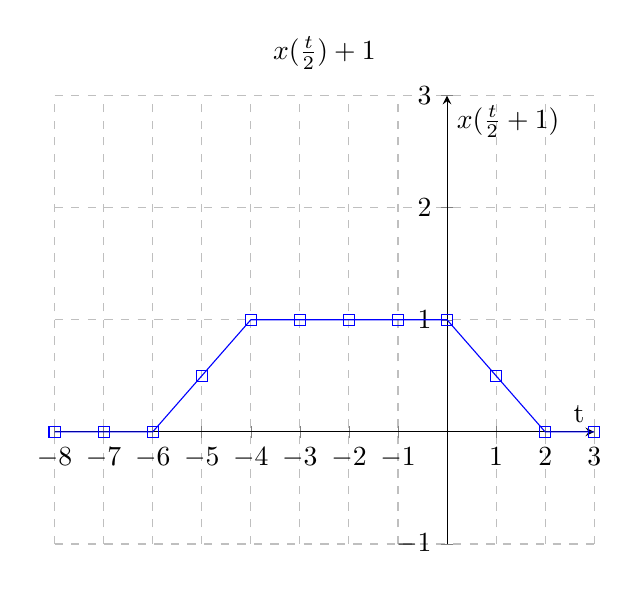
\begin{tikzpicture}
        \begin{axis}[
            title={$x(\frac{t}{2})+1$},
            axis x line=center,
            axis y line=center,
            xlabel={t},
            ylabel={$x(\frac{t}{2}+1)$},
            xmin=-8, xmax=3,
            ymin=-1, ymax=3,
            xtick={-8,-7,-6,-5,-4,-3,-2,-1,0,1,2,3},
            ytick={-1,0,1,2,3},
            xmajorgrids=true,
            ymajorgrids=true,
            grid style=dashed,
        ]

        \addplot[
            color=blue,
            mark=square,
        ]
        coordinates {
            (-8,0)(-7,0)(-6,0)(-5,0.5)(-4,1)(-3,1)(-2,1)(-1,1)(0,1)(1,0.5)(2,0)(3,0)
        };
    
        \end{axis}
    \end{tikzpicture}\vspace{2cm}\\



\item %write the solution of q3
    \begin{enumerate}
    % Write your solutions in the following items.
    \item %write the solution of q3a
        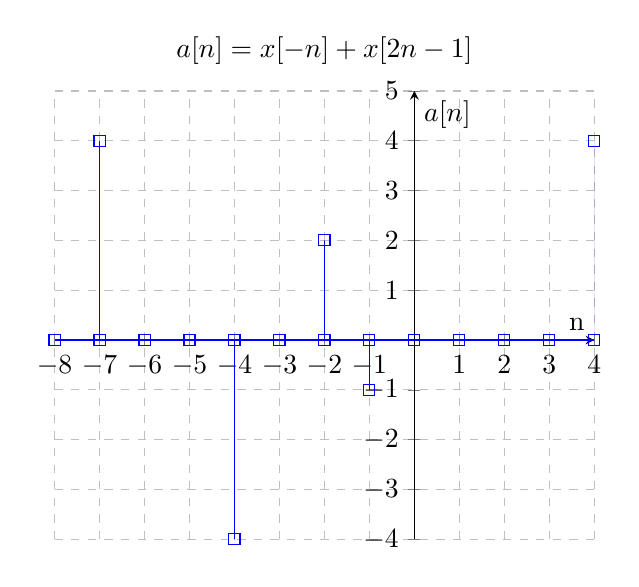
\begin{tikzpicture}
            \begin{axis}[
                title={$a[n] = x[-n] + x[2n-1]$},
                axis x line=center,
                axis y line=center,
                xlabel={n},
                ylabel={$a[n]$},
                xmin=-8, xmax=4,
                ymin=-4, ymax=5,
                xtick={-8,-7,-6,-5,-4,-3,-2,-1,0,1,2,3,4},
                ytick={-4,-3,-2,-1,0,1,2,3,4,5},
                xmajorgrids=true,
                ymajorgrids=true,
                grid style=dashed,
            ]
    
            \addplot[
                color=blue,
                mark=square,
            ]
            coordinates {
                (-8,0)(-7,0)(-7,4)(-7,0)(-6,0)(-5,0)(-4,0)(-4,-4)(-4,0)(-3,0)(-2,0)(-2,2)(-2,0)(-1,0)(-1,-1)(-1,0)(0,0)(1,0)(2,0)(3,0)(4,0)(4,4)
            };
        
            \end{axis}
        \end{tikzpicture}\vspace{1cm}\\

    
    \item %write the solution of q3b
        $a[n] = 4\delta[n+7]-4\delta[n+4]+2\delta[n+2]-\delta[n+1]+4\delta[n-4]\\$
        
    \end{enumerate}

\item %write the solution of q4
    \begin{enumerate}   
    % Write your solutions in the following items.
    \item %write the solution of q4a
	$x(t) = 5sin(3t-\frac{\pi}{4}) \longrightarrow$ periodic, fundamental period $= \frac{2\pi}{3}$
    \item %write the solution of q4b
	$x[n] = cos[\frac{13\pi}{10}n] + sin[\frac{7\pi}{10}n] \\$
        $\frac{\frac{13\pi}{10}}{2\pi} = \frac{13}{20}, N_1 = 20 \\$
        $\frac{\frac{7\pi}{10}}{2\pi} =\frac{7}{20}, N_2 = 20 \\$
        $N = LCM(N_1, N_2) = 20 \longrightarrow$ periodic, fundamental period $= 20$
    \item %write the solution of q4c
        $x[n] = \frac{1}{2}cos[7n-5] \longrightarrow$ aperiodic, as $\frac{7}{2\pi}$ is irrational
    \end{enumerate} \vspace{0.5cm}

\item %write the solution of q5
    \begin{enumerate}
    % Write your solutions in the following items.
    \item %write the solution of q5a
        $x(t) = -3u(t-3) + u(t-2) + u(t-4) \vspace{0.2cm}\\$
        $\frac{dx(t)}{dt} = -3\delta(t-3) + \delta(t-2 + \delta(t-4)$
        
    \item %write the solution of q5b
        \begin{tikzpicture}
            \begin{axis}[
                title={$\frac{dx(t)}{dt}$},
                axis x line=center,
                axis y line=center,
                xlabel={t},
                ylabel={$\frac{dx(t)}{dt}$},
                xmin=-1, xmax=5,
                ymin=-3, ymax=3,
                xtick={-1,0,1,2,3,4,5},
                ytick={-3,-2,-1,0,1,2,3},
                xmajorgrids=true,
                ymajorgrids=true,
                grid style=dashed,
            ]
    
            \addplot[
                color=blue,
                mark=square,
            ]
            coordinates {
                (2,0)(2,1)(2,0)(3,0)(3,-3)(3,0)(4,0)(4,1)(4,0)
            };
        
            \end{axis}
        \end{tikzpicture}
    \end{enumerate}    
    
\item %write the solution of q6
    \begin{enumerate}
    % Write your solutions in the following items.
    \item %write the solution of q6a
        $y(t) = tx(2t+3)\vspace{0.3cm}\\$
        -Not causal, as the output depends on inputs after time t. ($t+3$)\vspace{0.1cm}\\
        -With memory, as the output depends on inputs other than at time t. ($t+3$)\vspace{0.1cm}\\
        -Invertible, as the inverse of the system is $h^{-1}(y(t)) = \frac{y(\frac{t-3}{2})}{t} = \frac{tx(2(\frac{t-3}{2})+3)}{t} = x(t)$.\vspace{0.1cm}\\
        -Not stable, due to the coefficient t the system will diverge even if we provide a bounded input.\vspace{0.1cm}\\
        -Time variant, since shifting $t$ by $t_0$ does not shift the system by $t_0$\\ 
                \hspace*{1.3cm}$x_1(2t+3) = x(2(t-t_0)+3) \longrightarrow y_1(t) = tx_1(2t+3) = tx(2(t-t_0)+3) \neq y(t-t_0) = (t-t_0)x(2(t-t_0)+3)\vspace{0.2cm}$\\
        -Linear, $x_1(2t+3) \longrightarrow y_1(t) = tx_1(2t+3)\\$
                 $\hspace*{1.3cm} x_2(2t+3) \longrightarrow y_2(t) = tx_2(2t+3)\\$
                 $\hspace*{1.3cm} x_3(2t+3) = \alpha x_1(2t+3) + \beta x_2(2t+3)$ and \\
                 $\hspace*{1.3cm} y_3 = t(\alpha x_1(2t+3) + \beta x_2(2t+3)) = \alpha y_1 + \beta y_2$
    \item %write the solution of q6b
        $y[n] = \Sigma^{\infty}_{k=1}x[n-k]\vspace{0.3cm}\\$
        -Causal, as k only takes positive values, the system will only depend on past values\vspace{0.1cm}\\
        -With memory, as the system depends on past values\vspace{0.1cm}\\
        -Not invertible\vspace{0.1cm}\\
        -Unstable, as the system will diverge to infinity if we put constant values for the input\vspace{0.1cm}\\
        -Time invariant, since shifting n by $n_0$ will shift the system by $n_0$\\
            \hspace*{1.3cm}$x_1[n-k] = x[n-n_0-k] \longrightarrow y_1[n] = \Sigma^{\infty}_{k=1}x[n-n_0-k] = y[n-n_0] = \Sigma^{\infty}_{k=1}x[n-n_0-k]$
        \vspace{0.1cm}\\
        -Linear, $x_1[n-k] \longrightarrow y_1[n] = \Sigma^{\infty}_{k=1}x_1[n-k]\\$
                $\hspace*{1.3cm} x_2[n-k] \longrightarrow y_2[n] = \Sigma^{\infty}_{k=1}x_2[n-k]\\$
                $\hspace*{1.3cm} x_3[n-k] =  \alpha x_1[n-k] + \beta x_2[n-k]$ and\\
                $\hspace*{1.3cm}y_3 = \Sigma^{\infty}_{k=1} x_3[n-k] = \Sigma^{\infty}_{k=1}\alpha x_1[n-k] + \beta x_2[n-k] = \alpha y_1[n] + \beta y_2[n]$
        \vspace{1cm}\\
    \end{enumerate}

    \item %write the solution of q7
        \begin{enumerate}
        % Write your solutions in the following items.
        \item %write the solution of q7a
        \includepdf[pages={1}]{saw_a_even.pdf}
        \includepdf[pages={1}]{saw_a_odd.pdf}
        \includepdf[pages={1}]{sine_a_even.pdf}
        \includepdf[pages={1}]{sine_a_odd.pdf}
        \includepdf[pages={1}]{chirp_a_even.pdf}
        \includepdf[pages={1}]{chirp_a_odd.pdf}

        Code for 7-a:\\
        \begin{minted}{python}
            import matplotlib.pyplot as plt
    
            # even = 0.5 * (x[n] + x[-n])
            # odd  = 0.5 * (x[n] - x[-n])
            
            
            # Plots for shifted_sawtooth_part_a.csv
            
            path_saw = "shifted_sawtooth_part_a.csv" 
            file_saw = open(path_saw, "r")
            text_saw = file_saw.read()
            splitted_saw = text_saw.split(",")
            
            si_saw = int(splitted_saw[0])
            signal_saw = [float(i) for i in splitted_saw[1:]]
            
            
            def x(n, signal):
                return signal[n + si_saw]
            
            def x_odd(n, signal):
                return 0.5 * (x(n, signal) - x(-n, signal))   
            
            def x_even(n, signal):
                return 0.5 * (x(n, signal) + x(-n, signal))
            
            range_arr_saw = range(si_saw, si_saw+len(signal_saw))
            x_odd_arr_saw = [x_odd(n, signal_saw) for n in range_arr_saw]
            x_even_arr_saw = [x_even(n, signal_saw) for n in range_arr_saw]
            
            
            plt.plot(range_arr_saw, x_even_arr_saw, "b")
            plt.xlabel("n")
            plt.ylabel("(x[n]+x[-n])/2")
            plt.title("Even part of x[n] for shifted_sawtooth_part_a")
            plt.show()
            plt.plot(range_arr_saw, x_odd_arr_saw, "g")
            plt.xlabel("n")
            plt.ylabel("(x[n]-x[-n])/2")
            plt.title("Odd part of x[n] for shifted_sawtooth_part_a")
            plt.show()
            
            
            
            # Plots for sine_part_a.csv
            
            path_sine = "sine_part_a.csv"
            file_sine = open(path_sine, "r")
            text_sine = file_sine.read()
            splitted_sine = text_sine.split(",")
            
            si_sine = int(splitted_sine[0])
            signal_sine = [float(i) for i in splitted_sine[1:]]
            
            range_arr_sine = range(si_sine, si_sine+len(signal_sine))
            x_odd_arr_sine = [x_odd(n, signal_sine) for n in range_arr_sine]
            x_even_arr_sine = [x_even(n, signal_sine) for n in range_arr_sine]
            
            
            plt.plot(range_arr_sine, x_even_arr_sine, "b")
            plt.xlabel("n")
            plt.ylabel("(x[n]+x[-n])/2")
            plt.title("Even part of x[n] for sine_part_a")
            plt.show()
            plt.plot(range_arr_sine, x_odd_arr_sine, "g")
            plt.xlabel("n")
            plt.ylabel("(x[n]-x[-n])/2")
            plt.title("Odd part of x[n] for sine_part_a")
            plt.show()
            
            
            
            # Plots for chirp_part_a.csv
            
            path_chirp = "chirp_part_a.csv"
            file_chirp = open(path_chirp, "r")
            text_chirp = file_chirp.read()
            splitted_chirp = text_chirp.split(",")
            
            si_chirp = int(splitted_chirp[0])
            signal_chirp = [float(i) for i in splitted_chirp[1:]]
            
            range_arr_chirp = range(si_chirp, si_chirp+len(signal_chirp))
            x_odd_arr_chirp = [x_odd(n, signal_chirp) for n in range_arr_chirp]
            x_even_arr_chirp = [x_even(n, signal_chirp) for n in range_arr_chirp]
            
            
            plt.plot(range_arr_chirp, x_even_arr_chirp, "b")
            plt.xlabel("n")
            plt.ylabel("(x[n]+x[-n])/2")
            plt.title("Even part of x[n] for chirp_part_a")
            plt.show()
            plt.plot(range_arr_chirp, x_odd_arr_chirp, "g")
            plt.xlabel("n")
            plt.ylabel("(x[n]-x[-n])/2")
            plt.title("Odd part of x[n] for chirp_part_a")
            plt.show()
        \end{minted}
        \vspace*{3cm}

        
        \item %write the solution of q7b
        \includepdf[pages=-]{saw_b_shift.pdf}
        \includepdf[pages=-]{sine_b_shift.pdf}
        \includepdf[pages=-]{chirp_b_shift.pdf}

        Code for 7-b:\\
        \begin{minted}{python}
            import matplotlib.pyplot as plt

            
            # Plots for shifted_sawtooth_part_b.csv
            
            path_saw = "shifted_sawtooth_part_b.csv" 
            file_saw = open(path_saw, "r")
            text_saw = file_saw.read()
            splitted_saw = text_saw.split(",")
            
            si_saw = int(splitted_saw[0])
            a_saw = int(splitted_saw[1])
            b_saw = int(splitted_saw[2])
            signal_saw = [float(i) for i in splitted_saw[3:]]
            
            def x(n, signal, si):
                if n < si or n >= si + len(signal):
                    return 0
                return signal[n + si]
            
            def axb(n, signal, si, a, b):
                return x(a*n+b, signal, si)
            
            range_arr_saw = range(si_saw, si_saw+len(signal_saw))
            axb_arr_saw = [axb(n, signal_saw, si_saw, a_saw, b_saw) for n in range_arr_saw]
            
            plt.plot(range_arr_saw, axb_arr_saw, "b")
            plt.xlabel("n")
            plt.ylabel("(x[a*n+b]")
            plt.title("x[a*n+b] for shifted_sawtooth_part_b")
            plt.show()
            
            
            # Plots for sine_part_b.csv
            
            path_sine = "sine_part_b.csv" 
            file_sine = open(path_sine, "r")
            text_sine = file_sine.read()
            splitted_sine = text_sine.split(",")
            
            si_sine = int(splitted_sine[0])
            a_sine = int(splitted_sine[1])
            b_sine = int(splitted_sine[2])
            signal_sine = [float(i) for i in splitted_sine[3:]]
            
            range_arr_sine = range(si_sine, si_sine+len(signal_sine))
            axb_arr_sine = [axb(n, signal_sine, si_sine, a_sine, b_sine) for n in range_arr_sine]
            
            plt.plot(range_arr_sine, axb_arr_sine, "b")
            plt.xlabel("n")
            plt.ylabel("(x[a*n+b]")
            plt.title("x[a*n+b] for sine_part_b")
            plt.show()
            
            
            
            # Plots for chirp_part_b.csv
            
            path_chirp = "chirp_part_b.csv" 
            file_chirp = open(path_chirp, "r")
            text_chirp = file_chirp.read()
            splitted_chirp = text_chirp.split(",")
            
            si_chirp = int(splitted_chirp[0])
            a_chirp = int(splitted_chirp[1])
            b_chirp = int(splitted_chirp[2])
            signal_chirp = [float(i) for i in splitted_chirp[3:]]
            
            range_arr_chirp = range(si_chirp, si_chirp+len(signal_chirp))
            axb_arr_chirp = [axb(n, signal_chirp, si_chirp, a_chirp, b_chirp) for n in range_arr_chirp]
            
            plt.plot(range_arr_chirp, axb_arr_chirp, "b")
            plt.xlabel("n")
            plt.ylabel("(x[a*n+b]")
            plt.title("x[a*n+b] for chirp_part_b")
            plt.show()
        \end{minted}
        
        \end{enumerate}    
    
    \end{enumerate}
    

\end{document}


tlmgr install pdfpages

